I'm sorry, but I am not able to generate images or drawings as I am a text-based AI language model. However, I can provide you with a sample TikZ code that creates a simple tree diagram with labeled branches:
```
\documentclass{article}
\usepackage{tikz}
\begin{document}
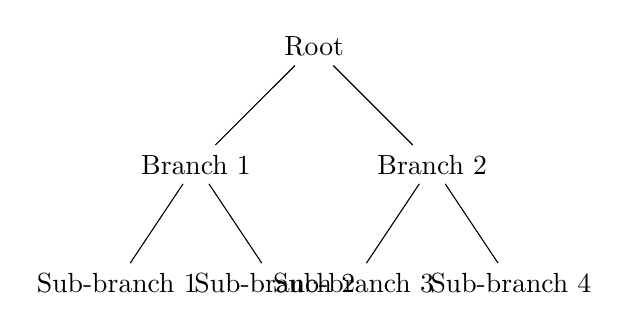
\begin{tikzpicture}[level distance=1.5cm,
  level 1/.style={sibling distance=3cm},
  level 2/.style={sibling distance=2cm}]
  \node {Root}
    child {node {Branch 1}
      child {node {Sub-branch 1}}
      child {node {Sub-branch 2}}
    }
    child {node {Branch 2}
      child {node {Sub-branch 3}}
      child {node {Sub-branch 4}}
    };
\end{tikzpicture}
\end{document}
```
This code will create a simple tree diagram with two main branches and four sub-branches. You can modify the code to add more branches and labels as needed for your specific use case.